\chapter{需求建模}
\section{数据流图}
\subsection{顶层数据流图}
\subsection{0层数据流图}
\begin{figure}[H]
\centering
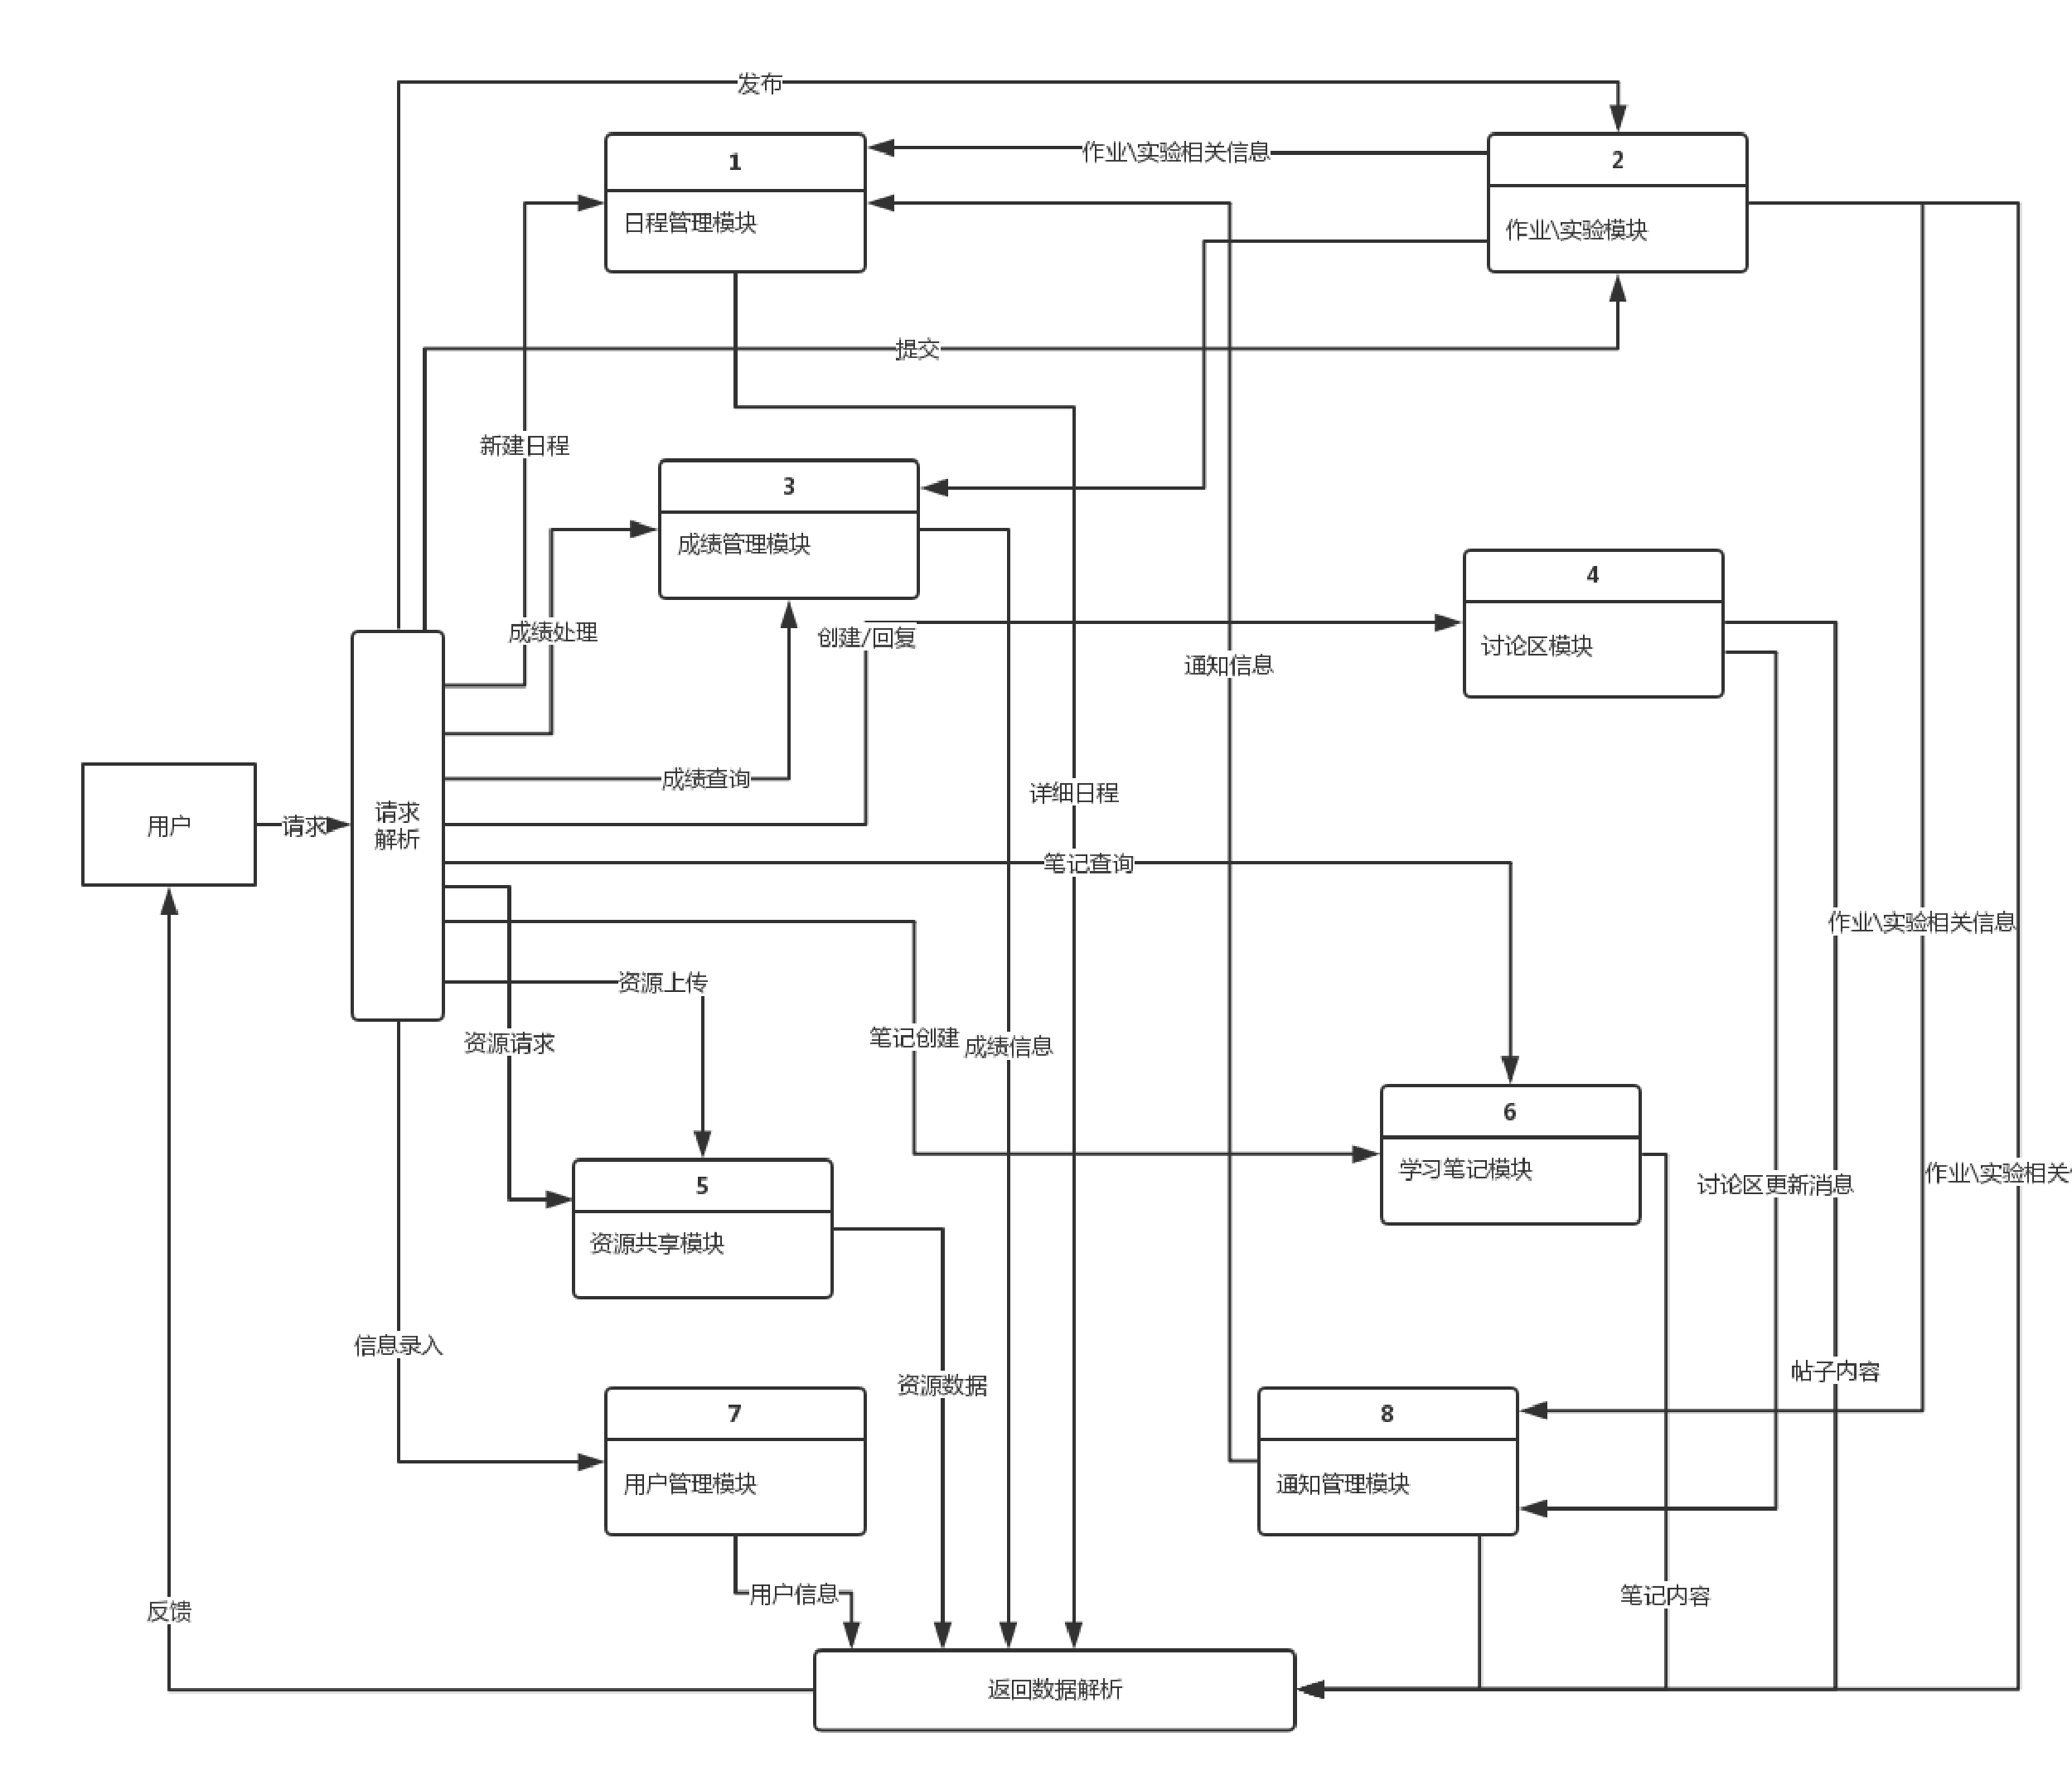
\includegraphics[width=18cm]{Level_0}
\caption{0层数据流图}
\end{figure}
\subsection{1层数据流图}
\subsubsection{日程管理模块}
\begin{figure}[H]
\centering
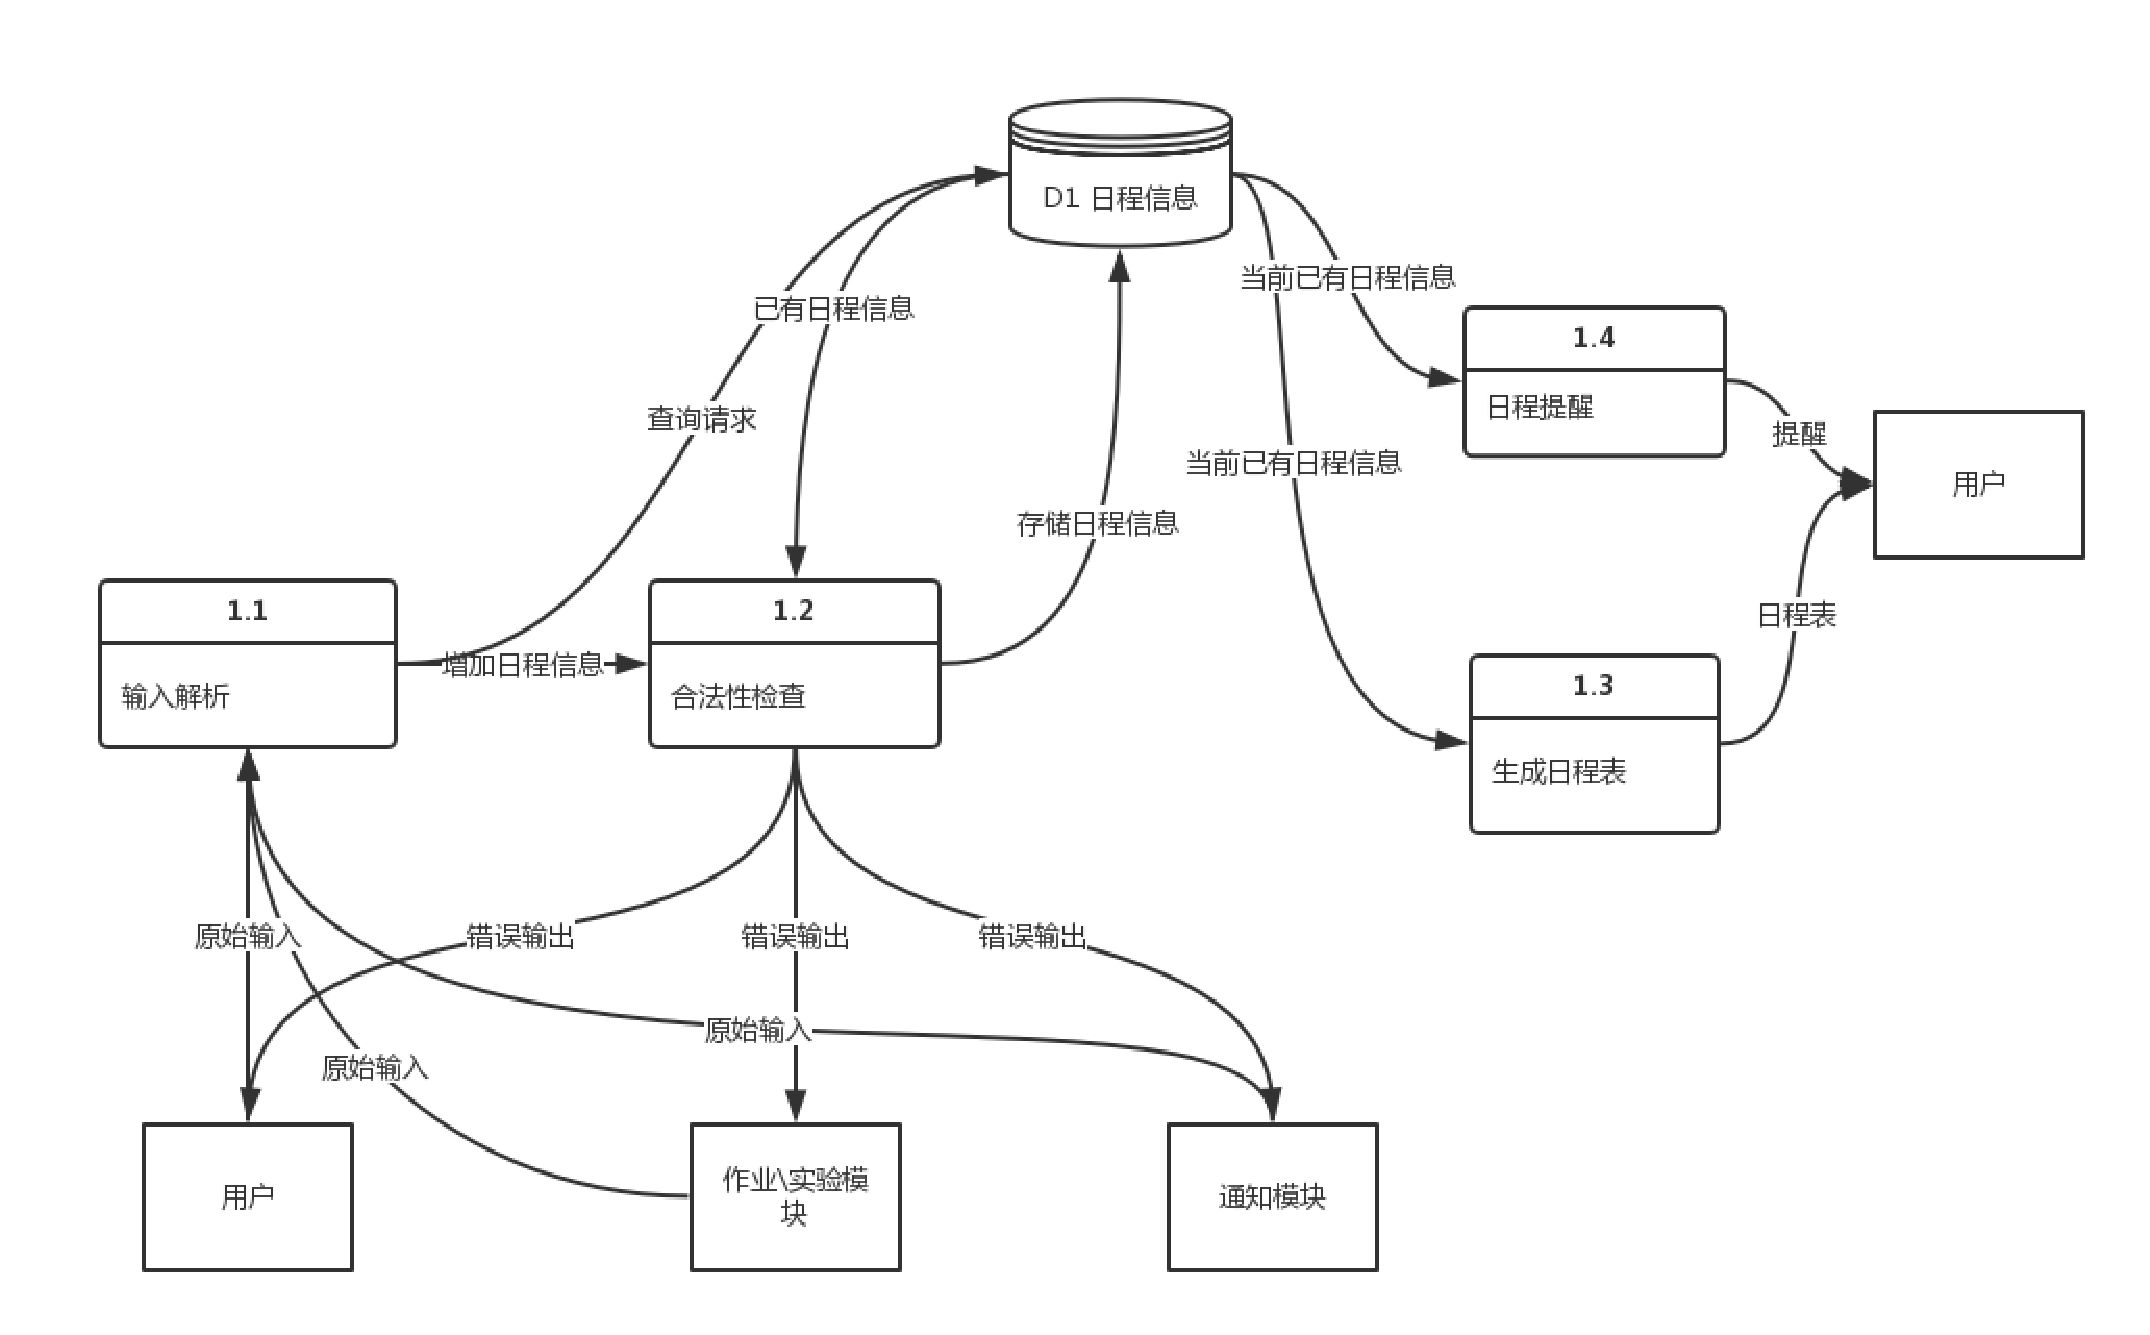
\includegraphics[width=15cm]{level1_日程管理}
\caption{日程管理模块功能数据流图}
\end{figure}
\subsubsection{作业实验模块}
\begin{figure}[H]
\centering
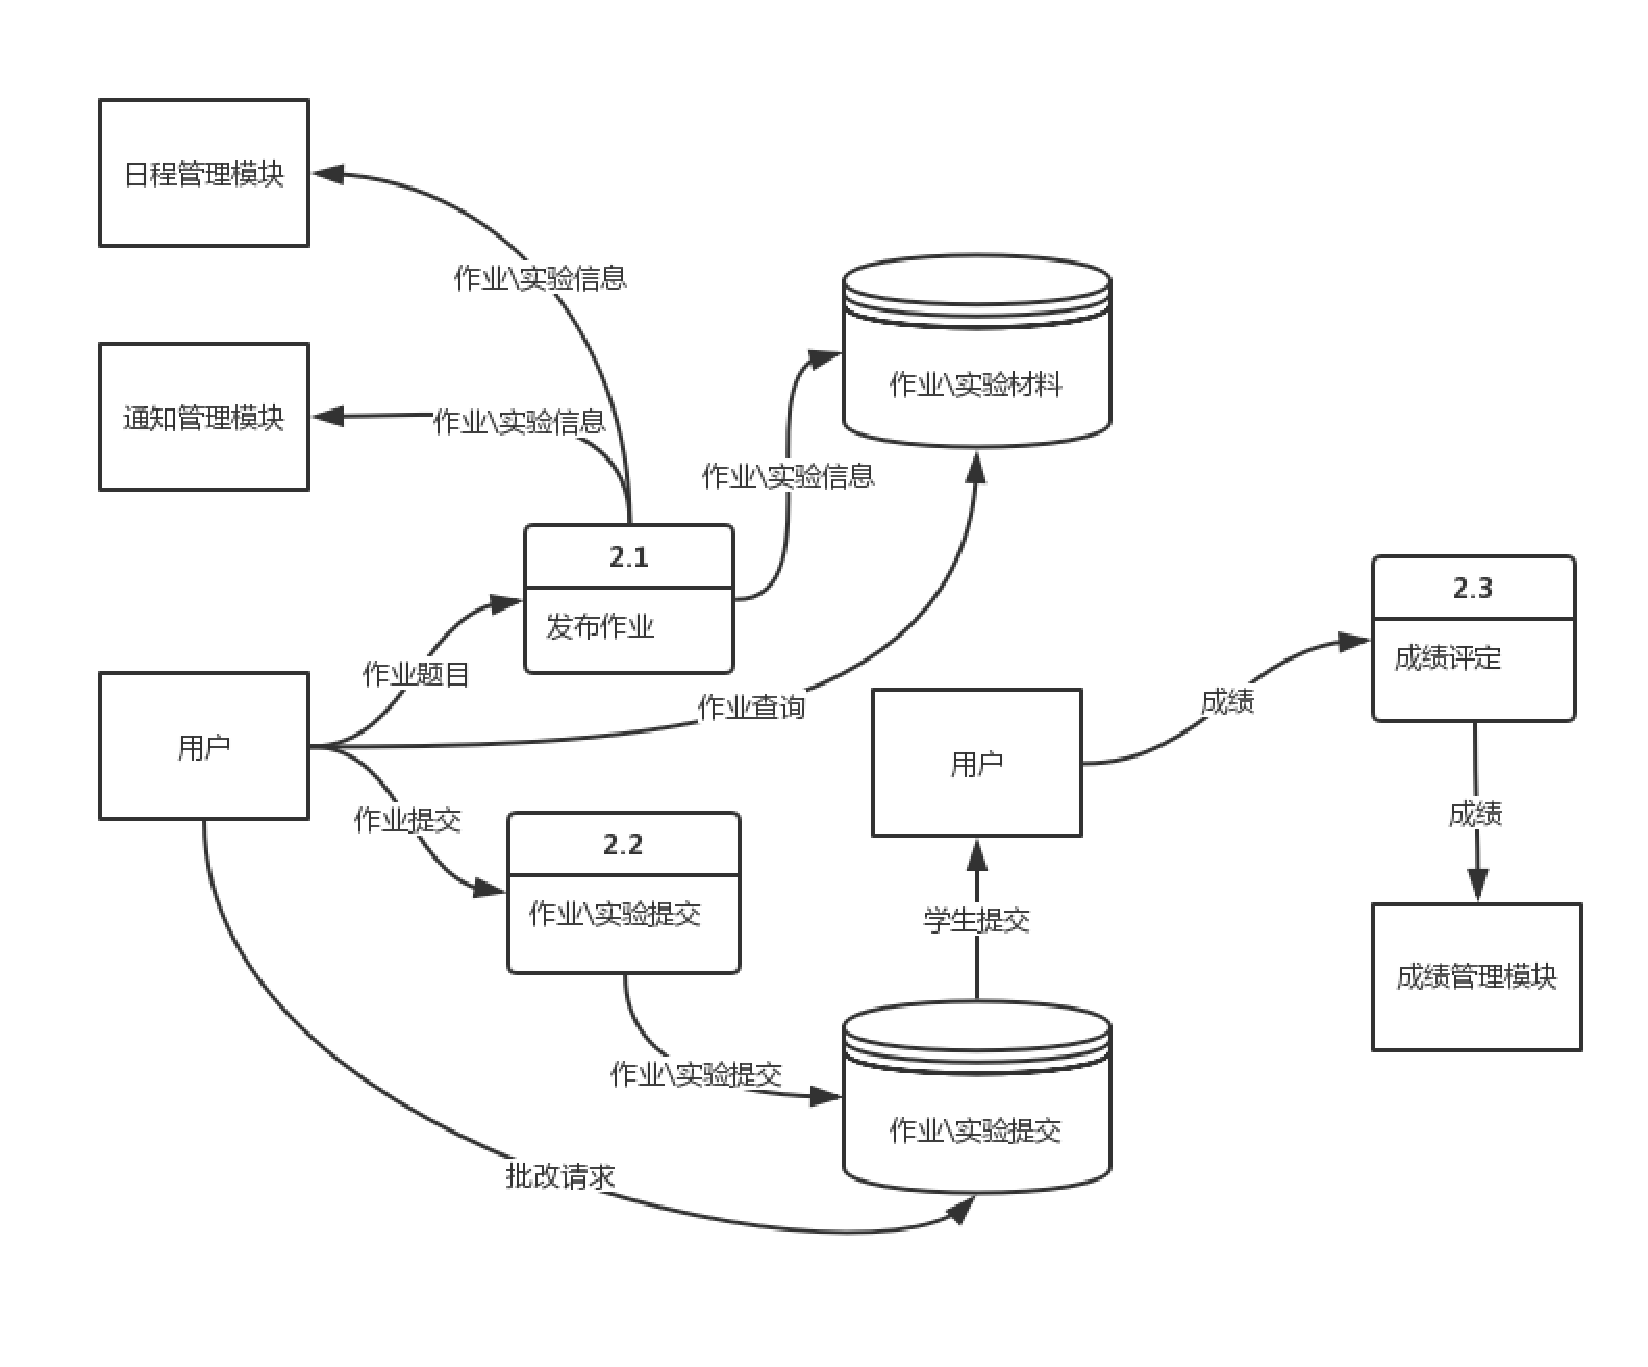
\includegraphics[width=15cm]{level1_作业}
\caption{日程管理模块功能数据流图}
\end{figure}
\subsubsection{学习笔记模块}
\begin{figure}[H]
\centering
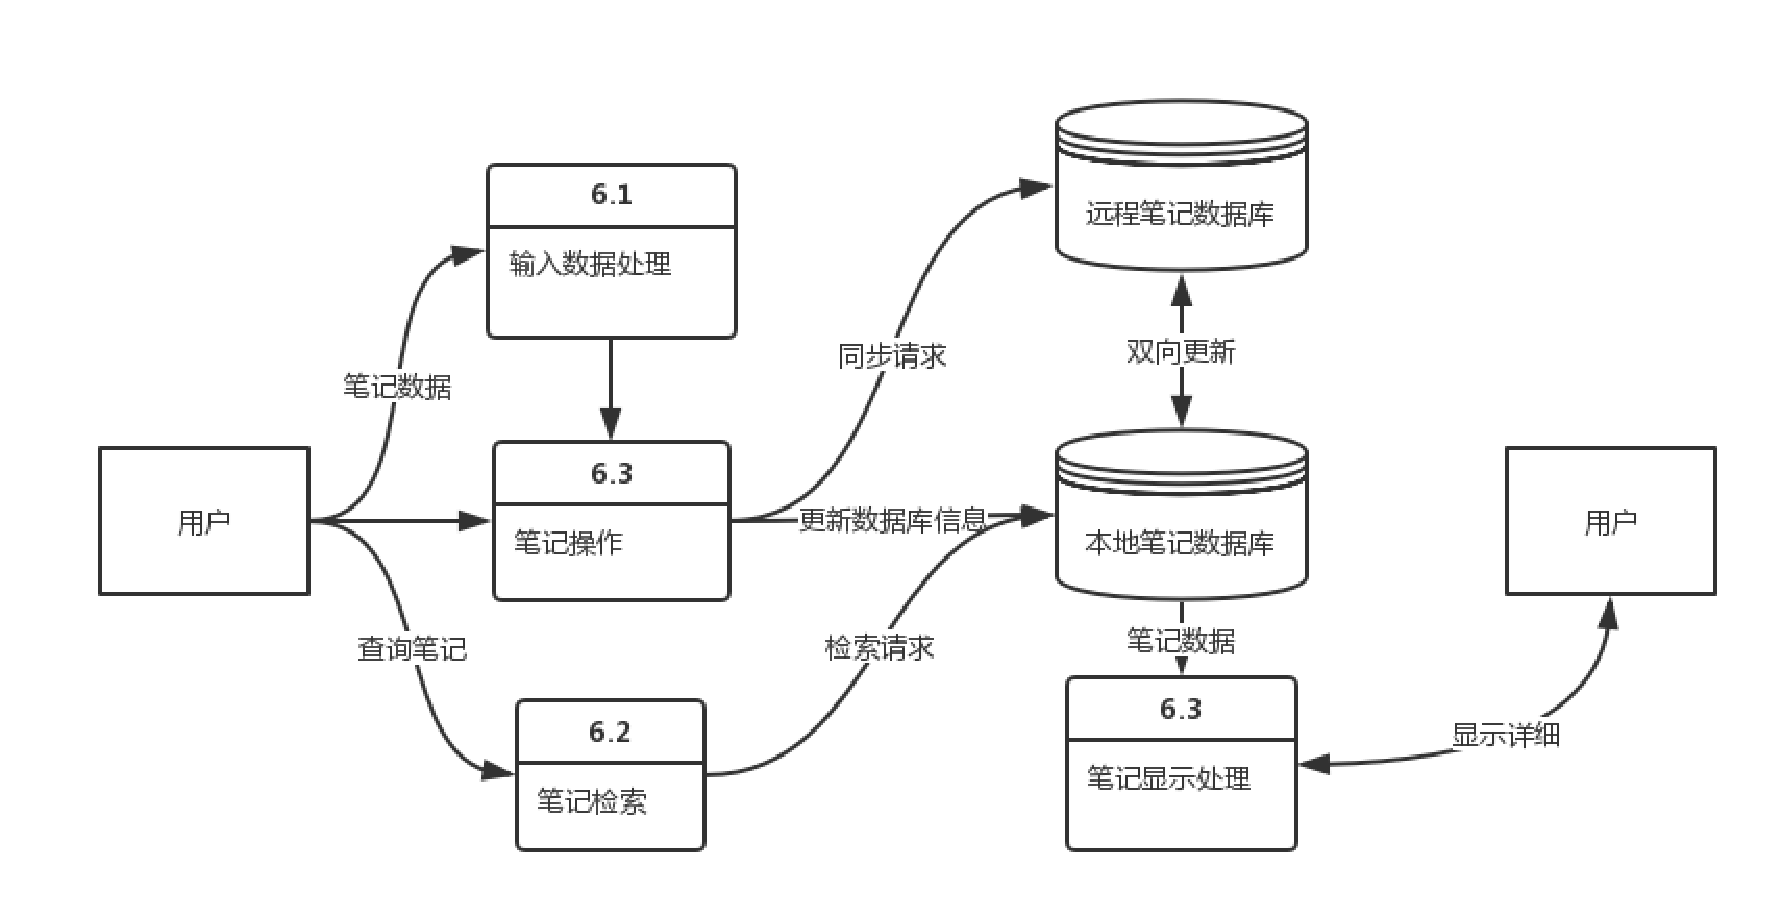
\includegraphics[width=15cm]{level1_学习笔记}
\caption{学习笔记模块功能数据流图}
\end{figure}
\subsubsection{成绩管理模块}
\begin{figure}[H]
\centering
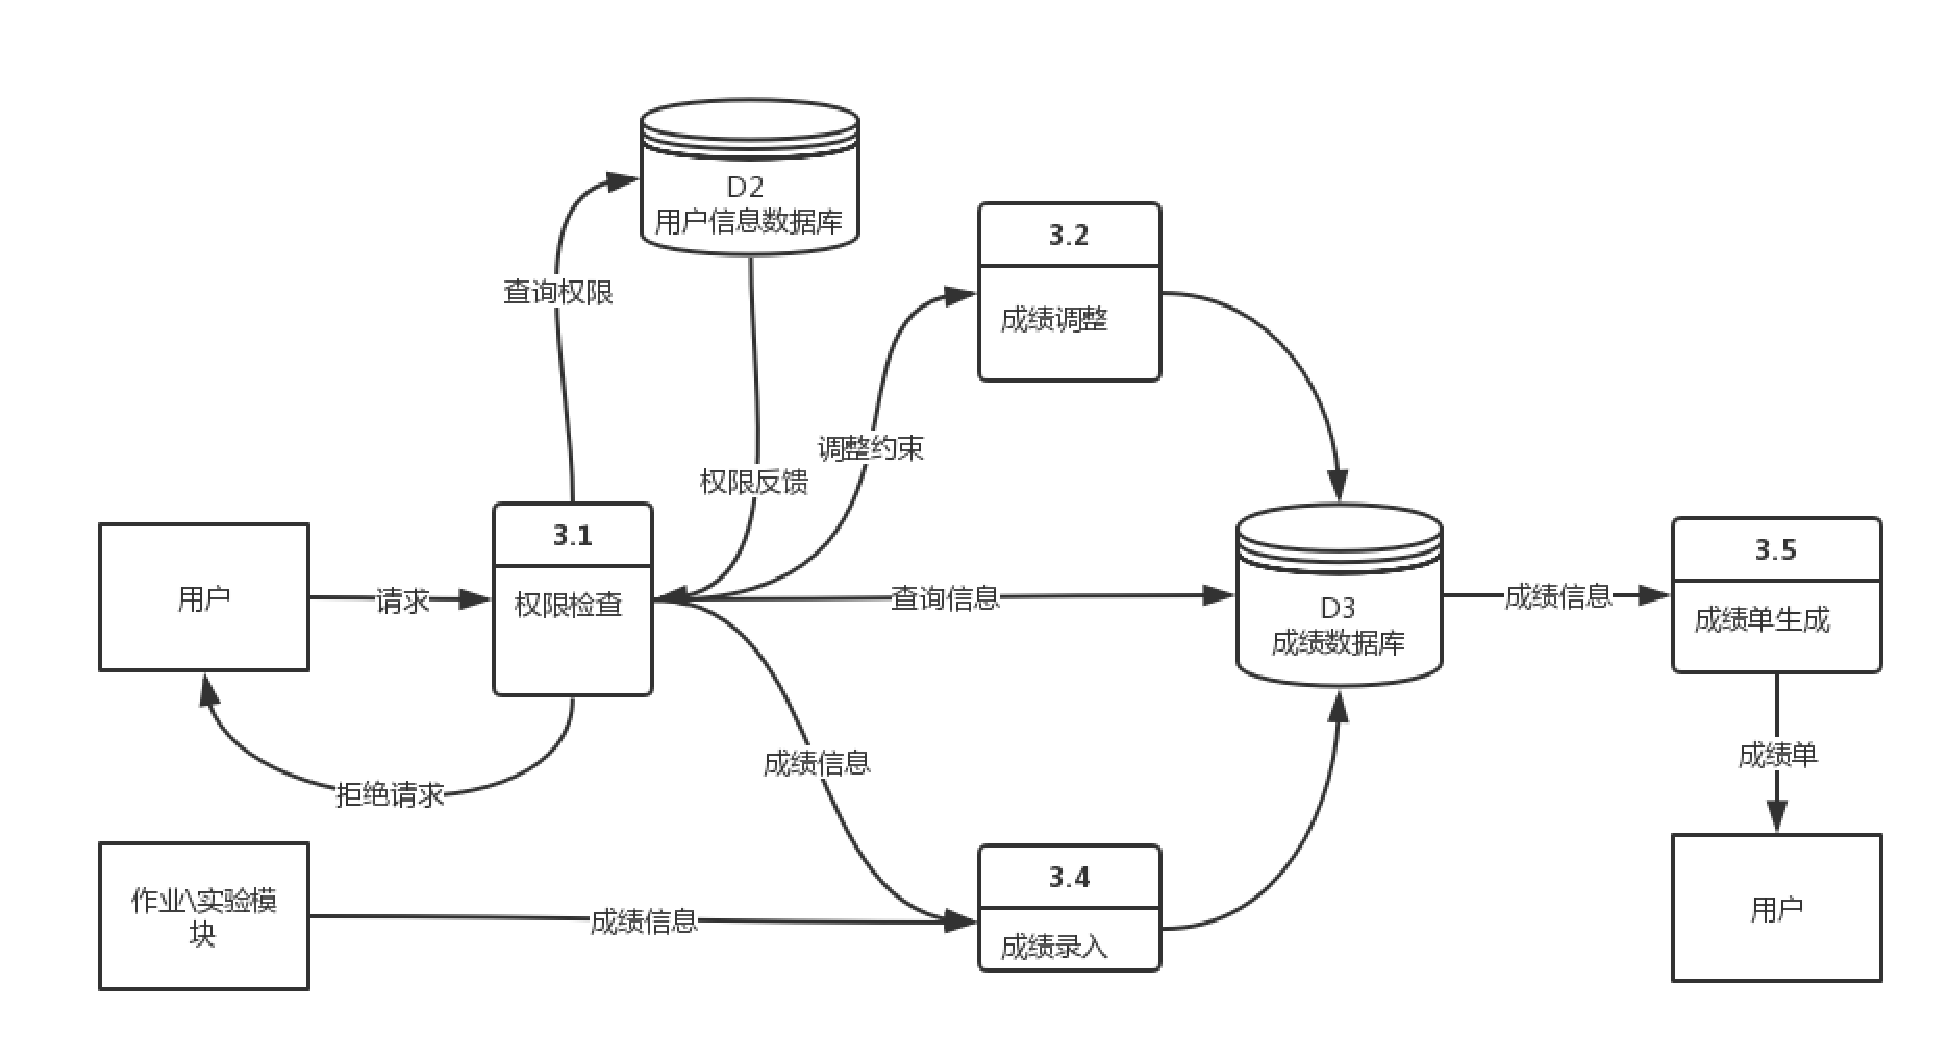
\includegraphics[width=15cm]{level1_成绩管理}
\caption{成绩管理模块功能数据流图}
\end{figure}
\subsubsection{用户管理模块}
\begin{figure}[H]
\centering
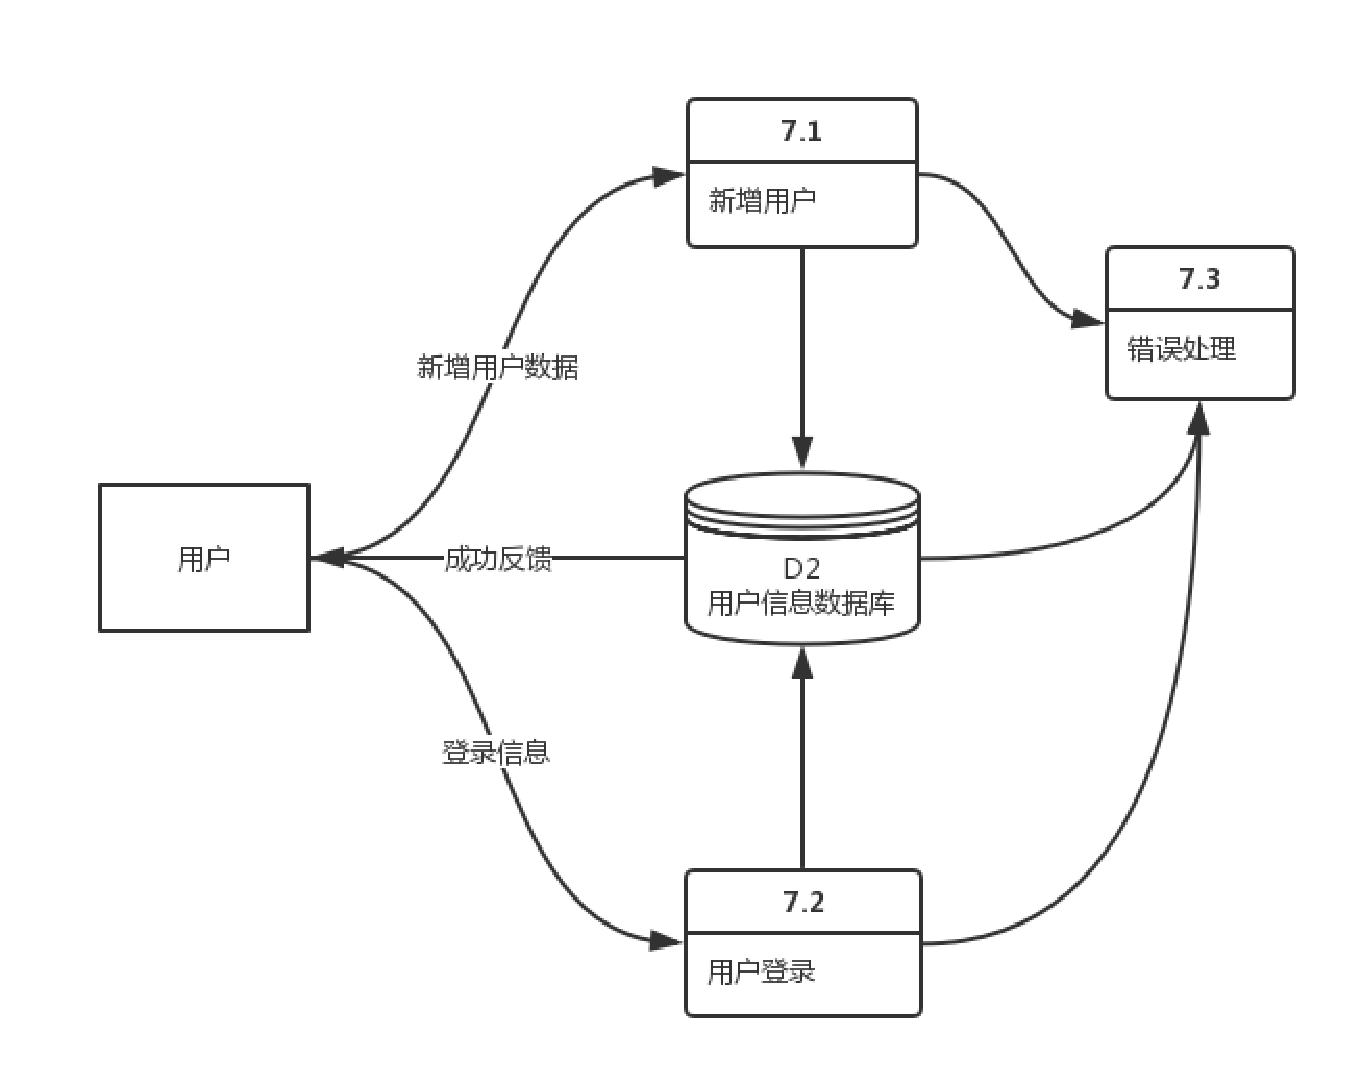
\includegraphics[width=15cm]{level1_用户管理}
\caption{用户理模块功能数据流图}
\end{figure}
\subsubsection{讨论区模块}
\begin{figure}[H]
\centering
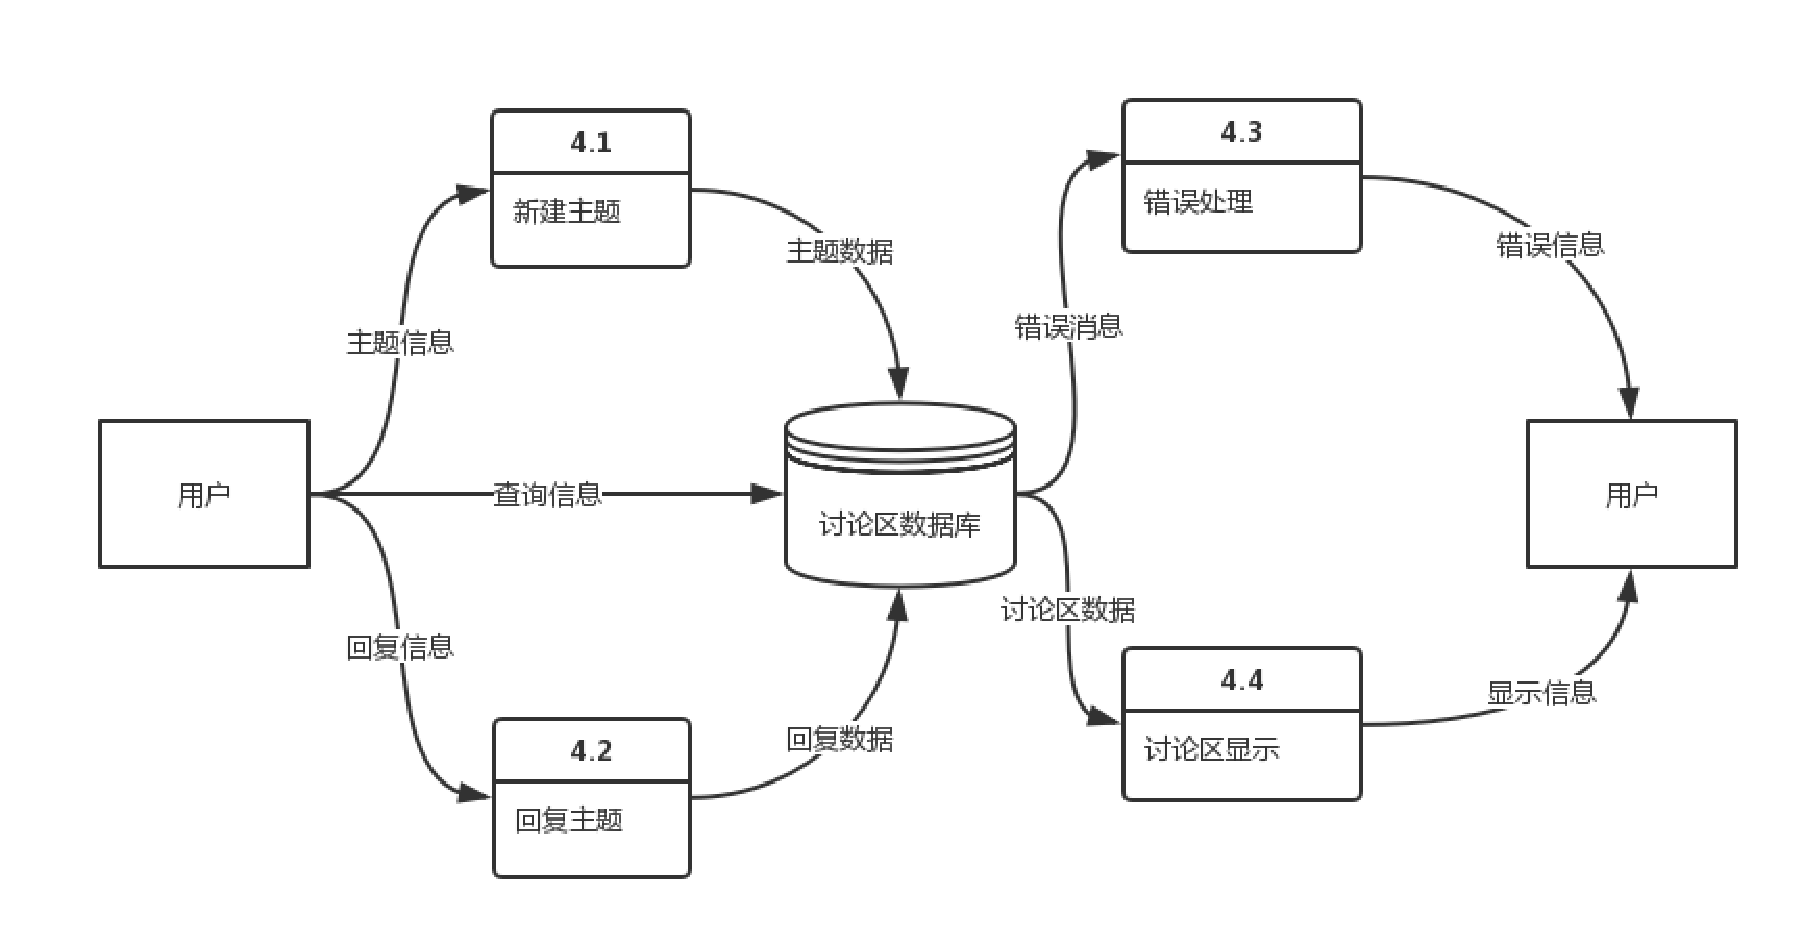
\includegraphics[width=15cm]{level1_讨论区}
\caption{讨论区模块功能数据流图}
\end{figure}
\subsubsection{资源共享模块}
\begin{figure}[H]
\centering
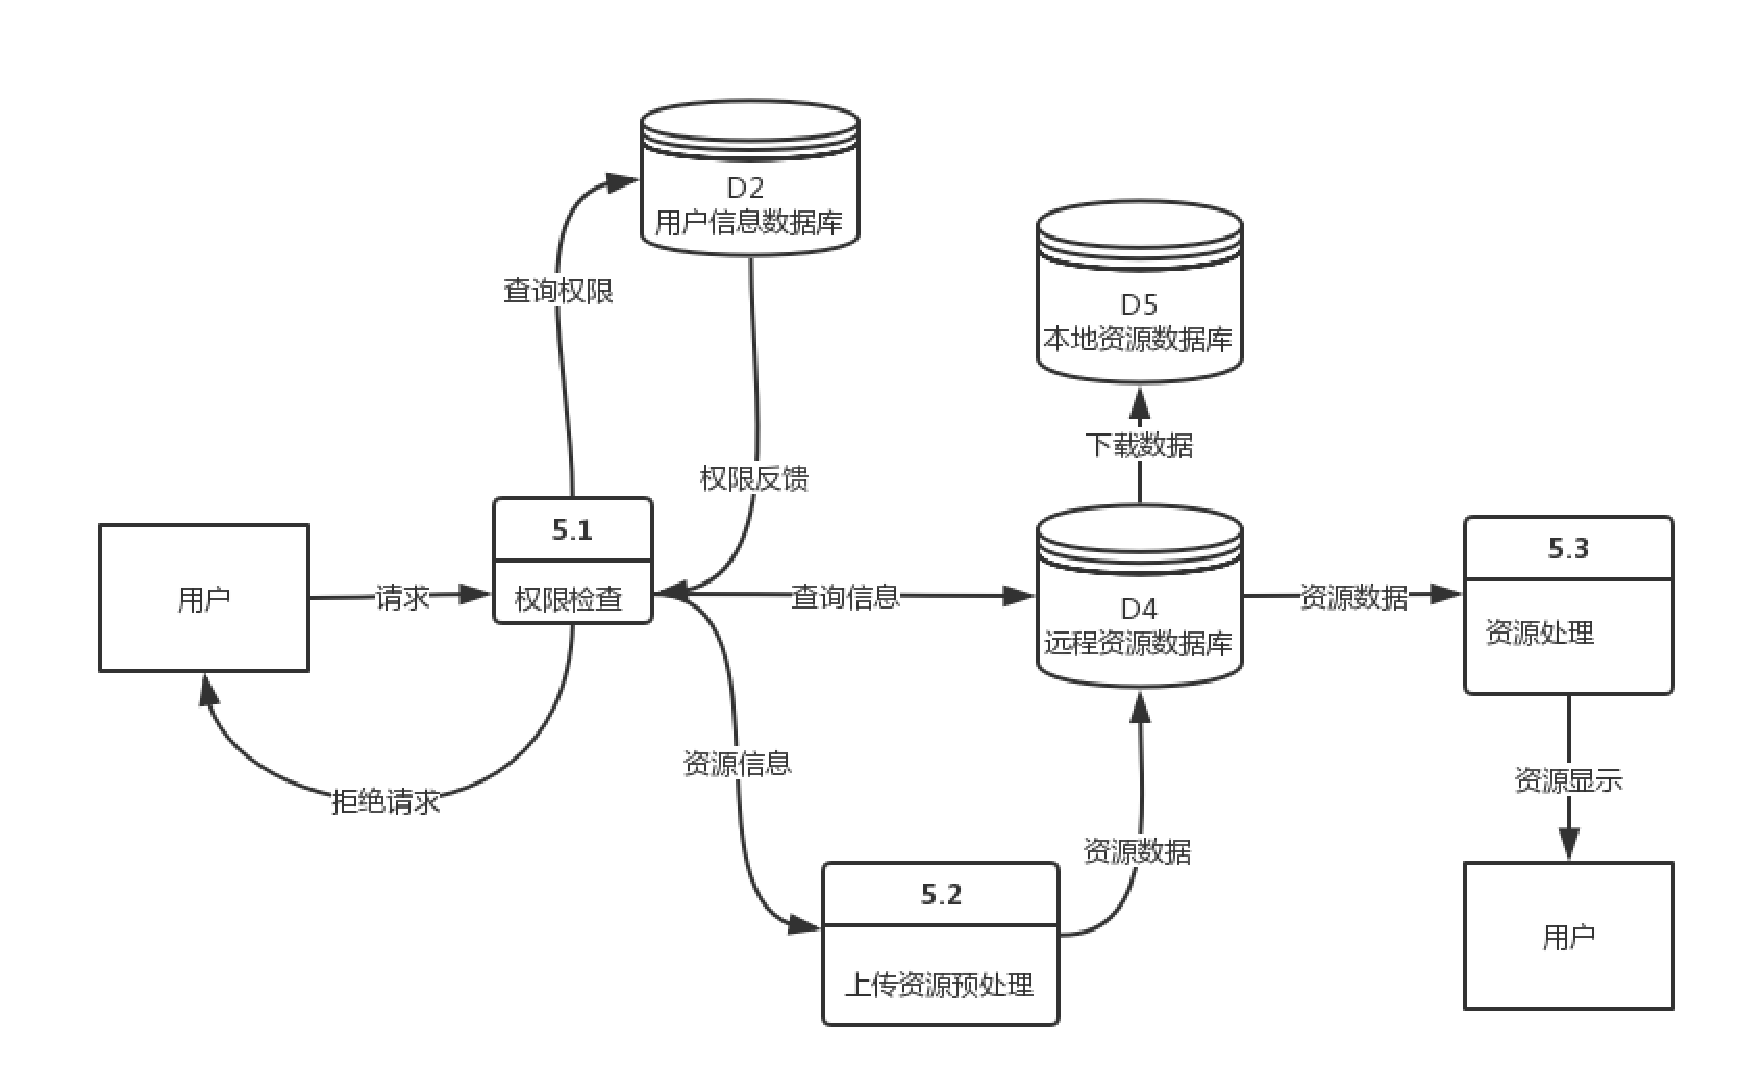
\includegraphics[width=15cm]{level1_资源共享}
\caption{资源共享模块功能数据流图}
\end{figure}
\subsubsection{通知管理模块}
\begin{figure}[H]
\centering
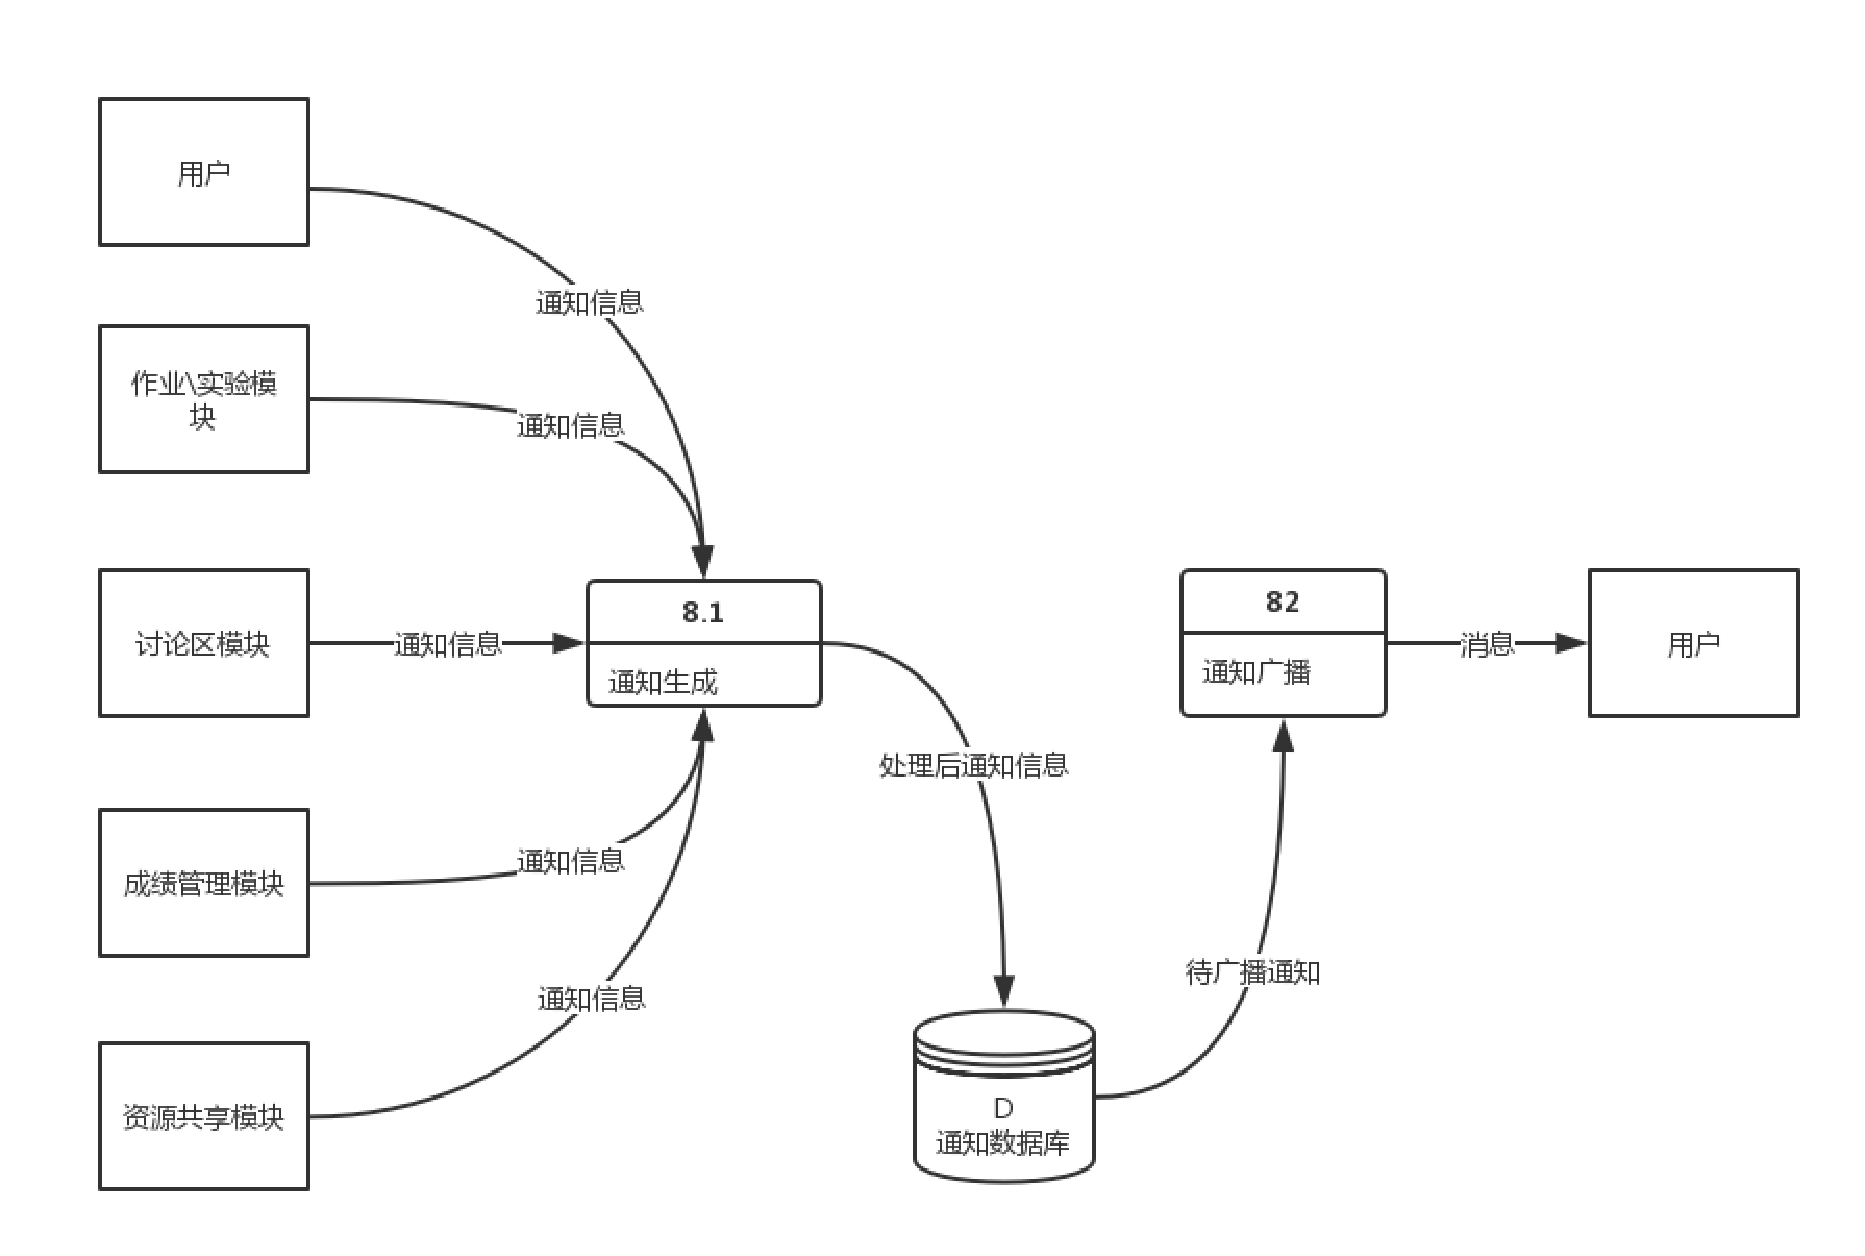
\includegraphics[width=15cm]{level1_通知管理}
\caption{通知管理模块功能数据流图}
\end{figure}

\section{数据字典}
\subsection{数据流说明}
\subsubsection{请求}
来源:用户
简述:用户对数据“请求操作”
去向:请求解析

\subsubsection{信息录入}
来源:请求解析
简介:讲用户信息录入数据库
去向:用户管理模块

\subsubsection{用户信息}
来源:用户管理模块
简介:从数据库中导出的用户信息
去向:返回数据解析

\subsubsection{反馈}
来源:返回数据解析
简介:客户端对于用户数据的处理结果
去向:用户

\subsubsection{作业/实验/通知查询}
来源:用户
简介:对作业/实验进行查询请求
去向:作业/实验材料,日程管理模块,通知模块

\subsubsection{作业/实验/通知发布}
来源:用户
简介:新的作业/实验创建
去向:发布作业

\subsubsection{作业/实验/通知提交}
来源:用户
简介:提交作业
去向:作业/实验提交

\subsubsection{作业/实验查看与批改}
来源:请求解析
简介:查看学生提交的作业
去向:用户,本地数据库

\subsubsection{笔记创建}
来源:请求解析
简介:新的笔记条目的创建
去向:学习笔记模块

\subsubsection{笔记内容}
来源:学习笔记模块
简介:用户查询的笔记内容
去向:返回数据解析




\subsubsection{笔记数据}
来源:用户,本地笔记数据库
简介:用户的笔记内容
去向:输入数据处理,笔记操作,笔记显示处理

\subsubsection{查询笔记}
来源:用户
简介:对笔记数据进行查询请求
去向:笔记检索

\subsubsection{同步请求}
来源:笔记操作
简述:客户端与远程笔记同步
去向:远程笔记数据库

\subsubsection{更新数据库信息}
来源:笔记操作
简述:向客户端提出更新数据库命令
去向:本地笔记数据库

\subsubsection{双向更新}
来源:远程笔记数据库,本地笔记数据库
简述:客户端与远程笔记双向更新
去向:远程笔记数据库,本地笔记数据库

\subsubsection{检索请求}
来源:笔记检索
简述:在客户端查询笔记
去向:本地笔记数据库

\subsubsection{显示详细}
来源:笔记显示处理
简述:将笔记数据显示到用户界面
去向:用户

\subsubsection{新增用户数据}
来源:用户
简介:在数据库中增加用户
去向:新增用户

\subsubsection{成功反馈}
来源:用户信息数据库
简介:反馈给用户新增数据成功
去向:用户

\subsubsection{登录信息}
来源:用户,用户登录
简介:讲用户的登录信息在用户和客户端间同步
去向:用户,用户登录


\subsection{数据存储说明}
\subsubsection{数据库发布作业/实验/通知存储}
简述: 服务器数据库存放教师发布的作业/实验/通知

数据排列: 数据存在多个lable,主要的主键有发布课程编号,类型,作业号。其列名还有内容,截至日期,附件地址等。

\subsubsection{作业附件存储}
简述: 服务器存放教师发布的作业/实验材料

数据排列: 不同的科目有不同的文件夹,存放到相应的文件夹下。将地址存入数据库相应的部分。

\subsubsection{学生提交作业/实验存储}
简述: 服务器存放学生上传的作业/实验。

数据排列:数据库的主键为作业号。其列名还有学生学号,名称,作业/实验提交与否,地址。
将学生提交的内容存入服务器的文件夹下,地址放入上述服务器。

若使用git提交,则同样保存按照git服务器保存在服务器上。

\subsubsection{用户账号数据库存储}
\item简述:服务器端数据库存储用户的邮箱,学号,姓名,密码,用户权限,选修课程,课程详情等基本信息
\item数据排列:数据存在多个table,以用户邮箱,学生姓名,课程名称为主键,数据按主键排列

\subsubsection{笔记数据库存储}
\item简述:存储在服务器数据库中的用户信息,笔记内容,笔记创建时间,相关学科等信息
\item数据排列:数据存在多个table,数据以用户账户,笔记学科为主键,笔记按主键排列。

\subsubsection{笔记数据库本地存储}
\item简述:存储在客户端数据库中的笔记内容,笔记创建时间,相关学科等信息
\item数据排列:数据存在多个table,数据以笔记创建时间,笔记学科为主键,笔记按主键排列。

\subsection{加工说明}
\subsubsection{发布作业/实验/通知}
用户将作业/实验/通知填写好发送。

服务器判断用户发来的数据,将附件存入相应空间,将其他内容存入数据库中。

向客户端发送成功与否的信息。

\subsubsection{学生提交作业/实验}
学生将作业/实验内容从本地提交。

服务器接受消息,更新数据库,并将收到的文件存储。

向客户端发送结果信息。

\subsubsection{处理登录}
客户端发送查询请求到服务器用户数据库,匹配该用户邮箱或学号和密码,匹配成功则返回成功登录的信息,并同步数据。匹配失败则返回失败信息,并显示账户不存在或密码错误。

\subsubsection{处理新用户请求}
客户端发送新建请求到服务器数据库,检查是否为新用户,若可创建则返回允许创建信息,失败则返回无法创建新用户。

\subsubsection{处理笔记}
对笔记请求数据处理,分发给下一级功能区具体处理

\subsubsection{创建笔记}
创建新的笔记,创建成功则将新的笔记按用户选择存入本地存储,或存入服务器。

\subsubsection{删除笔记}
删除云端或者本地存储的笔记,返回操作结果。

\subsubsection{处理查询}
从本地存储和服务器存储的的数据文件进行搜索,对于符合关键字的搜索返回给用户,如果没有结果则显示无结果。
